\providecommand{\main}{../../../..}
\documentclass[\main/dresen_thesis.tex]{subfiles}
\begin{document}
  \label{sec:colloidalCrystals:layers:xrr}
  \begin{figure}[tb]
    \centering
    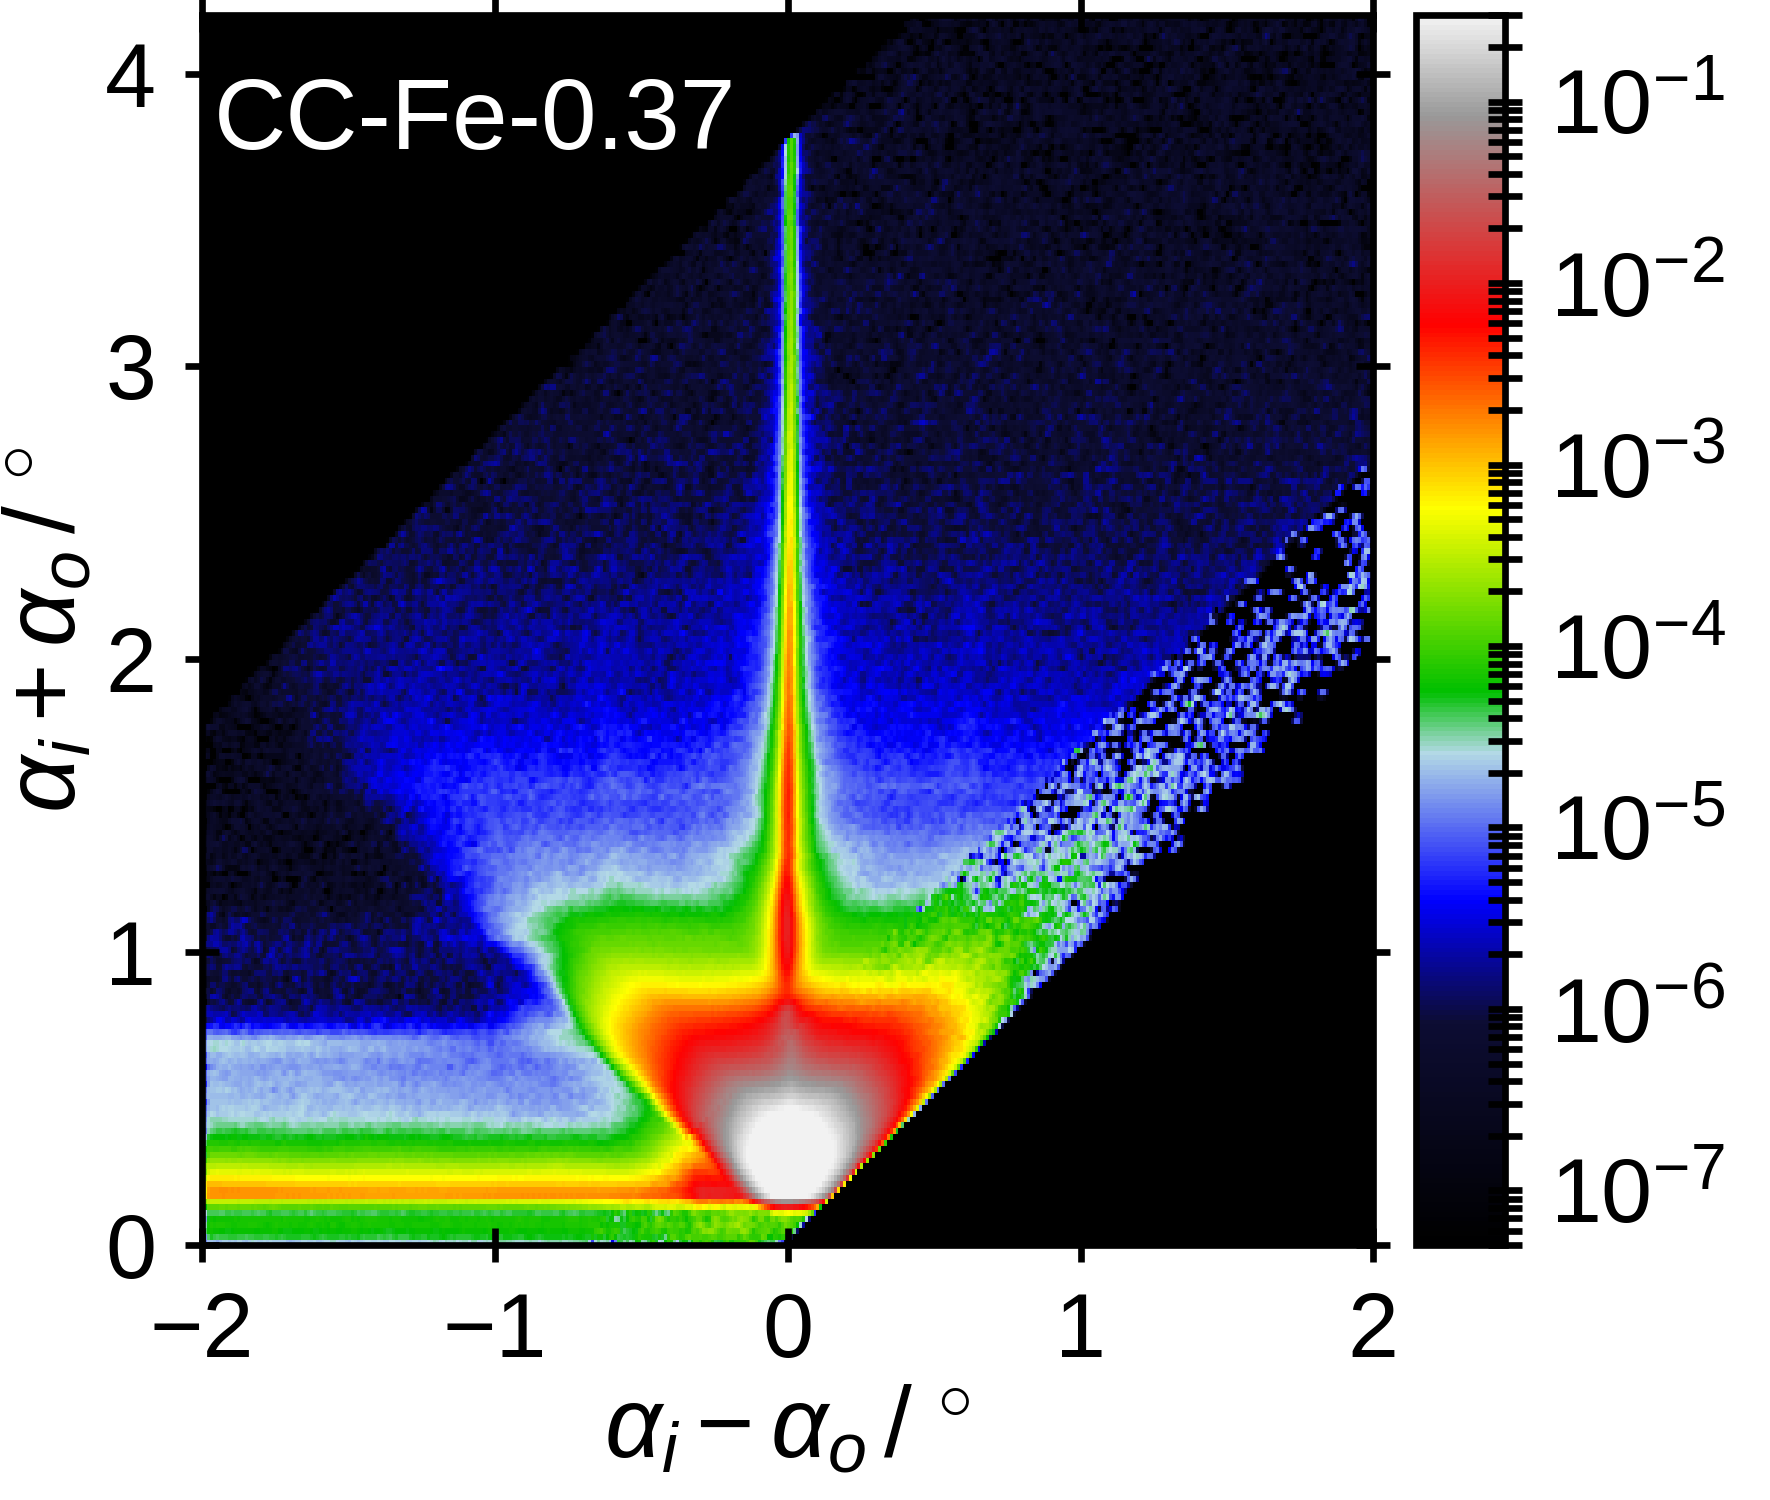
\includegraphics{colloidalCrystals_PNR_CC_Fe_0_37_ReflectivityMapXRR}
    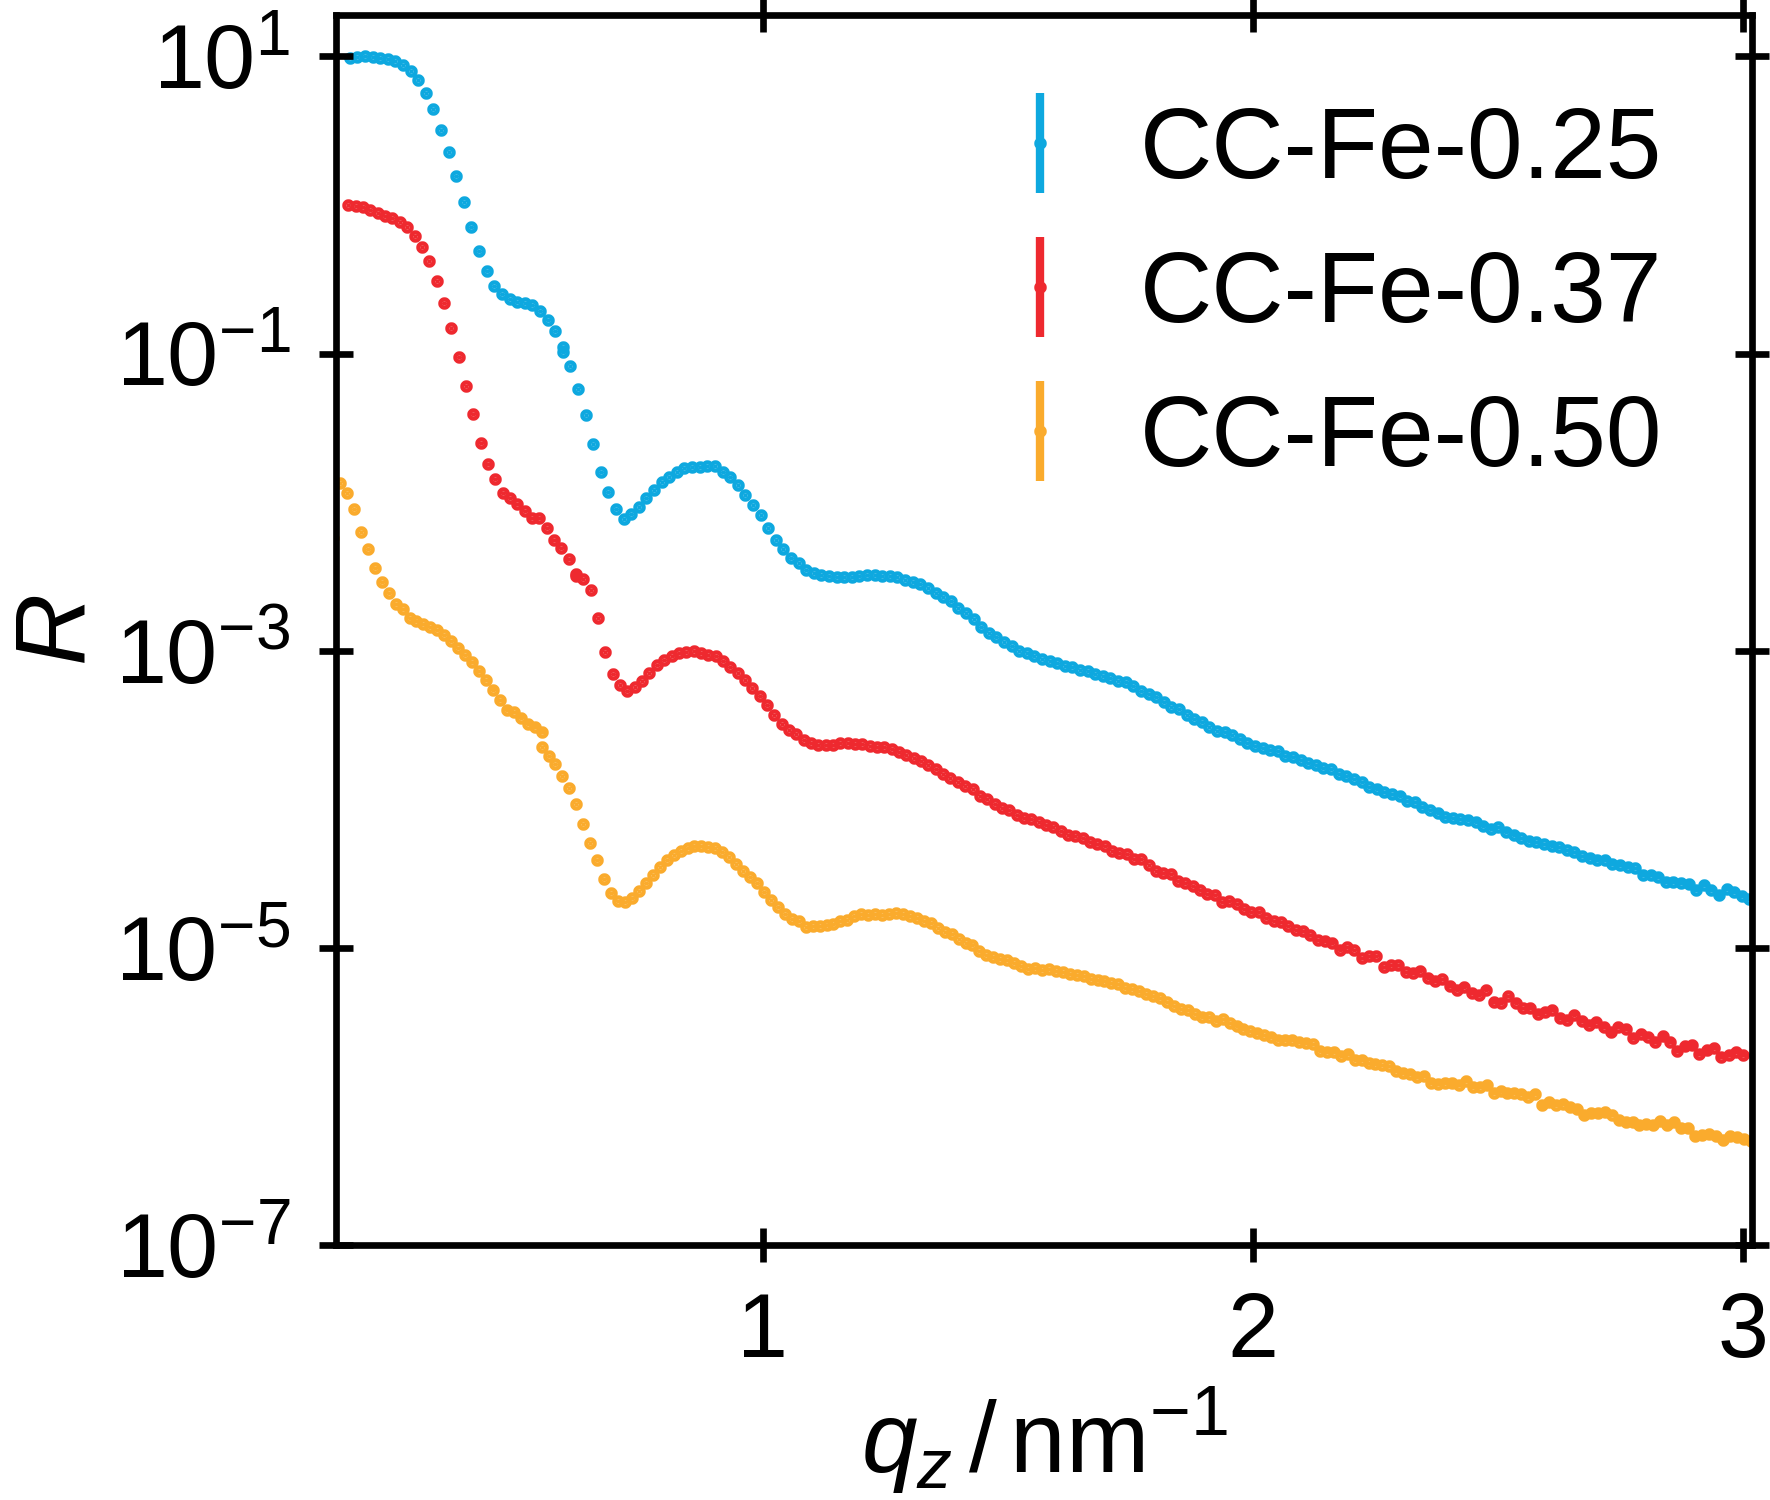
\includegraphics{colloidalCrystals_VerticalStructure_Combined_XRR}
    \caption{\label{fig:colloidalCrystals:xrr}X-ray reflectometry of CC-Fe-0.25, CC-Fe-0.37 and CC-Fe-0.50. Reducing the detector images, a reflectivity map is obtained, shown exemplarily for CC-Fe-0.37 (left). Integrating a box around $\alpha_i - \alpha_o \eq 0 ^\circ$ and subtracting the diffuse scattering from the off-specular region, the specular reflectivity is obtained (right). The reflectivities of the samples are scaled by a factor of ten respectively for distinction.}
  \end{figure}

  The three samples CC-Fe-0.25, CC-Fe-0.37 and CC-Fe-0.50 have been studied by X-ray reflectometry using the GALAXI instrument.
  An exemplary reflectivity map for CC-Fe-0.37 and the reflectivities of all samples are shown for direct comparison in \reffig{fig:colloidalCrystals:xrr}.
  The reflectivity map shows the specular reflectivity line around $\alpha_i - \alpha_o \eq 0 ^\circ$ as region of strong intensity and additionally broad Bragg sheets in the off specular region.
  Slightly visible in the reflectivity map is also the overlap region of the two data sets, which were measured with varied counting time, which is an artifact from the edge region of the respective data sets and cleaned from the integrated reflectivity.

  Qualitatively, the three reflectivities show similar features with a correlation peak near $0.53 \unit{nm^{-1}}$ and $0.87 \unit{nm^{-1}}$.
  With increasing sample thickness, the plateau of total reflection is bends down in direct comparison from CC-Fe-0.37 to CC-Fe-0.25 and is not visible for the case of CC-Fe-0.50.
  Also with increasing sample thickness, the first peak around $0.53 \unit{nm^{-1}}$ smears out and becomes less well-defined.

  The reduced critical edge can be argumented by the larger thickness of iron oxide nanocubes.
  The average scattering length density of the iron oxide layer can be lower than that of the silicon substrate and for an increasing thickness it becomes the determining density for the critical reflection condition.
  Additionally, iron oxide is partially absorbing for X-rays, which becomes apparent from the imaginary part of the scattering length density that is approximately $10 \%$ in magnitude of the real part.
  This leads to the observed rounding effect of the critical edge, where with increasing incident angle close to the critical edge the X-ray photons penetrate deeper into the layer and become partially absorbed.

  None of the reflectivities show defined Kiessig fringes, which could, however, still be expected from the observed sample thickness seen in SEM micrographs.
  Thus it can be concluded that a larger thickness variation is present in the sample, which would smear out the Kiessig fringes.

\end{document}